% This must be in the first 5 lines to tell arXiv to use pdfLaTeX, which is strongly recommended.
\pdfoutput=1
% In particular, the hyperref package requires pdfLaTeX in order to break URLs across lines.

\documentclass[11pt]{article}

% Change "review" to "final" to generate the final (sometimes called camera-ready) version.
% Change to "preprint" to generate a non-anonymous version with page numbers.
\usepackage[final]{acl}

% Standard package includes
\usepackage{times}
\usepackage{latexsym}

\usepackage{hyperref}
\usepackage{cleveref}

% \usepackage[utf8]{inputenc}
% \DeclareUnicodeCharacter{1DA4}{\fancyi}

% \newcommand\Istroke{\stroke{I}}

% For proper rendering and hyphenation of words containing Latin characters (including in bib files)
\usepackage[T1]{fontenc}
% For Vietnamese characters
% \usepackage[T5]{fontenc}
% See https://www.latex-project.org/help/documentation/encguide.pdf for other character sets

% This assumes your files are encoded as UTF8
\usepackage[utf8]{inputenc}

% This is not strictly necessary, and may be commented out,
% but it will improve the layout of the manuscript,
% and will typically save some space.
\usepackage{microtype}

% This is also not strictly necessary, and may be commented out.
% However, it will improve the aesthetics of text in
% the typewriter font.
\usepackage{inconsolata}

%Including images in your LaTeX document requires adding
%additional package(s)
\usepackage{graphicx}

\usepackage{tikz}
% \def\checkmark{\tikz\fill[scale=0.4](0,.35) -- (.25,0) -- (1,.7) -- (.25,.15) -- cycle;}
\newcommand{\tikzxmark}{%
\tikz[scale=0.23] {
    \draw[line width=0.7,line cap=round] (0,0) to [bend left=6] (1,1);
    \draw[line width=0.7,line cap=round] (0.2,0.95) to [bend right=3] (0.8,0.05);
}}
\newcommand{\tikzcmark}{%
\tikz[scale=0.23] {
    \draw[line width=0.7,line cap=round] (0.25,0) to [bend left=10] (1,1);
    \draw[line width=0.8,line cap=round] (0,0.35) to [bend right=1] (0.23,0);
}}

\usetikzlibrary{positioning, shapes.multipart}
\newcommand{\voc}[1]{\texttt{#1}}

\newcommand{\ensuretext}[1]{#1}
\newcommand{\nertcomment}[4]{\ensuretext{\textcolor{#3}{[\ensuretext{\textcolor{#3}{\ensuremath{^{\textsc{#1}}_{\textsc{#2}}}}} #4]}}}
\newcommand{\sw}[1]{\nertcomment{S}{W}{orange}{#1}}
\newcommand{\ejm}[1]{\nertcomment{E}{M}{green}{#1}}
\newcommand{\ri}[1]{\nertcomment{R}{I}{purple}{#1}}

% If the title and author information does not fit in the area allocated, uncomment the following
%
%\setlength\titlebox{<dim>}
%
% and set <dim> to something 5cm or larger.

\title{Can Uniform Meaning Representation Help GPT-4\\ Translate from Indigenous Languages?}

% Author information can be set in various styles:
% For several authors from the same institution:
% \author{Author 1 \and ... \and Author n \\
%         Address line \\ ... \\ Address line}
% if the names do not fit well on one line use
%         Author 1 \\ {\bf Author 2} \\ ... \\ {\bf Author n} \\
% For authors from different institutions:
% \author{Author 1 \\ Address line \\  ... \\ Address line
%         \And  ... \And
%         Author n \\ Address line \\ ... \\ Address line}
% To start a separate ``row'' of authors use \AND, as in
% \author{Author 1 \\ Address line \\  ... \\ Address line
%         \AND
%         Author 2 \\ Address line \\ ... \\ Address line \And
%         Author 3 \\ Address line \\ ... \\ Address line}

\author{Shira Wein \\
  Amherst College \\
  \texttt{swein@amherst.edu} }


\begin{document}
\maketitle
\begin{abstract}
While ChatGPT and GPT-based models are able to effectively perform many tasks without additional fine-tuning, they struggle with related to extremely low-resource languages and indigenous languages. 
Uniform Meaning Representation (UMR), a semantic representation designed to capture the meaning of texts in many languages, is well-poised to be leveraged in the development of low-resource language technologies.
In this work, we explore the downstream technical utility of UMR for low-resource languages by incorporating it into GPT-4 prompts.
Specifically, we examine the ability of GPT-4 to perform translation from three indigenous languages (Navajo, Arápaho, and Kukama), with and without demonstrations, as well as with and without UMR annotations. Ultimately we find that in the majority of our test cases, integrating UMR into the prompt results in a statistically significant increase in performance, which is a promising indication of future applications of the UMR formalism.
\end{abstract}

\section{Introduction}

\begin{figure}[t]
    % \small
% \begin{subfigure}
\centering
%\includegraphics[trim={0cm 1cm 0cm 0cm},clip, scale=0.4]{Unknown.png}
\resizebox{\linewidth}{!}{
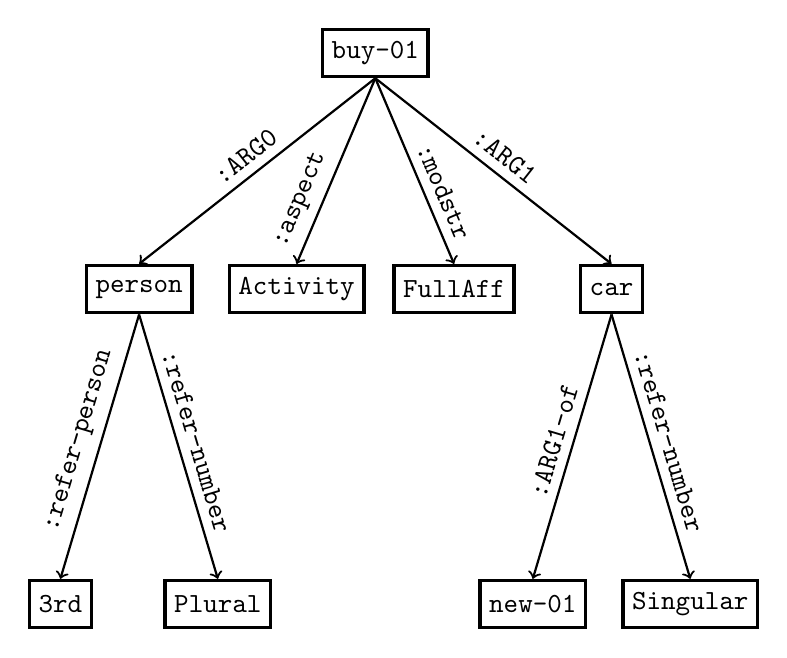
\begin{tikzpicture}[
blue/.style={rectangle, draw=black, very thick, minimum size=6mm},
]
	% Nodes
	\node[blue](s) at (10,10) {\voc{buy-01}};
	\node[blue](p) at (7,7) {\voc{person}};
    \node[blue](t) at (6,3) {\voc{3rd}};
    \node[blue](sing1) at (8,3) {\voc{Plural}};
	\node[blue](a) at (9,7) {\voc{Activity}};
	\node[blue](f) at (11,7) {\voc{FullAff}};
    \node[blue](c) at (13,7) {\voc{car}};
    \node[blue](sing2) at (14,3) {\voc{Singular}};
    \node[blue](n) at (12,3) {\voc{new-01}};
	% Edges
	\draw[->, thick] (s.south) -- (p.north) node[midway, above, sloped] {\voc{:ARG0}};
	\draw[->, thick] (s.south) -- (c.north) node[midway, above, sloped] {\voc{:ARG1}};
 	\draw[->, thick] (s.south) -- (a.north) node[pos=0.7, sloped, above] {\voc{:aspect}};
 	\draw[->, thick] (s.south) -- (f.north) node[pos=0.65, sloped, above] {\voc{:modstr}};
    \draw[->, thick] (c.south) -- (sing2.north) node[midway, above, sloped] {\voc{:refer-number}};
    \draw[->, thick] (c.south) -- (n.north) node[midway, above, sloped] {\voc{:ARG1-of}};
    \draw[->, thick] (p.south) -- (sing1.north) node[midway, above, sloped] {\voc{:refer-number}};
    \draw[->, thick] (p.south) -- (t.north) node[midway, above, sloped] {\voc{:refer-person}};

    
\end{tikzpicture}}
% \end{subfigure}
% \begin{subfigure}
\smallbreak
\small
\begin{verbatim}
(s / buy-01
  :ARG0 (p / person
    :refer-person 3rd
    :refer-number Plural)
  :ARG1 (c / car
    :ARG1-of (n / new-01)
    :refer-number Singular)
  :aspect Activity
  :modstr FullAff)
\end{verbatim}
% \end{subfigure}
\caption{UMR graph for the sentence ``They were buying a new car'' in both graph form (top) and in `PENMAN' notation \citep{kasper-1989-flexible}. 
% The `3rd' and `Singular' roles Note that 3rd and Singular are not concepts but attributes.
}
\label{fig:umr_example}
\end{figure}

% Uniform Meaning Representation (UMR) is a graph-based semantic representation designed to capture the core elements of meaning for a wide range of languages \citep{van2021designing}.
% UMR is based on Abstract Meaning Representation (AMR), which was designed for English 
% \citep{banarescu-etal-2013-abstract} but has since seen various cross-lingual extensions and applications \citep{10.1162/coli_a_00503}.
% In order to ensure that UMR could reflect meaning for many languages, the UMR schema is flexible in its annotation (via lattice-like language-dependent annotation) while ensuring consistency across languages. UMR also includes document-level graphs as well as the AMR-standard sentence-level graphs, enabling annotation of coreferential relations, and includes additional information such as aspect and modality.
% The UMR project has seen recent progress but is still in the early stages, with new resources such as an online web annotation tool \citep{ge-etal-2023-umr} and a relatively small recently-released annotated dataset \citep{bonn-etal-2024-building-broad}.


While ChatGPT models \citep{openai} are able to successfully produce text in many highly-resourced languages, they severely struggle with machine translation of low-resource languages
\citep{stap-araabi-2023-chatgpt,robinson-etal-2023-chatgpt}.

Uniform Meaning Representation \citep[UMR;][]{van2021designing} is a semantic representation created with the annotation of low-resource languages in mind.
The UMR formalism is designed to represent a wide range of languages by providing flexibility in the annotation process via paradigmatic lattices, and accommodates the annotation of extremely low-resource languages by creating the necessary linguistic resources (rolesets) during ``Stage 0'' of the annotation process.
UMR is a multilingual extension of the widely-adopted Abstract Meaning Representation \citep[AMR;][]{banarescu-etal-2013-abstract}.

The first UMR dataset \citep{bonn-etal-2024-building-broad} has recently been released, enabling exploration into the utility of UMR for tasks related to the generation of text into and from low-resource languages.
Recent work has also shown that GPT models likely do not implicitly contain the linguistic knowledge necessary to construct an AMR graph \citep{ettinger-etal-2023-expert}---or by extension, a UMR graph---suggesting that the addition of a UMR annotation may support prompt-based translation.

Thus, in this work, we explore the computational benefit of incorporating UMR graphs into ChatGPT prompts, specifically with regard to machine translation from extremely low-resource languages into English. 
Specifically, we craft four prompting protocols for GPT-4\footnote{\url{https://openai.com/index/gpt-4/}} which vary in both their number of demonstrations and whether UMR is included: zero-shot prompting, zero-shot prompting with the UMR graph of the text included, five-shot prompting, and five-shot prompting with the UMR graphs included.
We perform our experiments on three indigenous languages included in \citet{bonn-etal-2024-building-broad} (Navajo, Kukama, Arápaho), which also contain English references.
% \sw{shira to do: Contributions}
Our contributions include:
\begin{itemize}
\addtolength\itemsep{-2mm}
    \item Prompting protocols for translating from indigenous languages, with and without demonstrations (i.e. zero- and five-shot), and with and without UMR graphs of the source text. 
    \item GPT-based production of English translations of more than 1000 individual source sentences and their UMRs across three extremely-low resource languages, for each of our four prompting protocols.
    \item Statistical analyses of the results of each of our protocols, indicating the quantitative improvement resulting from the incorporation of UMR graphs and demonstrations.
\end{itemize}

\section{Background \& Related Work}

\subsection{Machine Translation with ChatGPT}

Recent work has explored the efficacy of prompting GPT models to generate text in no- and low-resource languages, with generally poor indications of success \citep{stap-araabi-2023-chatgpt}. 

Tackling the data sparsity issue, \citet{guo-etal-2024-teaching} propose a method for low-resource translation via ChatGPT and BLOOMZ \citep{muennighoff-etal-2023-crosslingual} by providing a vocabulary list and demonstrations as additional input.

Notably, \citet{robinson-etal-2023-chatgpt} find that ChatGPT performs competitively with state-of-the-art machine translation models for high-resource languages, but performs poorly for low-resource languages. In particular, the most significant predictor of ChatGPT translation performance on a language is the number of Wikipedia entries that exist in the language, serving as a proxy of how well-sourced that language is.

Additionally, five-shot prompts lead to small performance gains over zero-shot prompts.
\citet{tang2025adaptivefewshotpromptingmachine} further indicate that (in a high-resource setting) adaptive few-shot prompting, using the most semantically similar texts in the dataset to the source text as demonstrations, leads to further performance gains.
Related work has explored the general utility of chain-of-thought prompts for ChatGPT and found it to be ineffective, as it resulted in word-by-word translation \citep{peng-etal-2023-towards}.


\subsection{Uniform Meaning Representation}

Uniform Meaning Representation (UMR), an extension of the popular semantic representation AMR, is designed to be multilingual and contains information about the text at both the sentence- and document-level \citep{van2021designing}.

UMR accommodates a range of linguistic features in comparison to AMR \citep{wein-bonn-2023-comparing} through the integration of lattice-based annotation structures, allowing the annotator to select the level of granularity appropriate for the individual language  \citep{van-gysel-etal-2019-cross}.
UMR is also particularly well-suited to the annotation of low- and no-resource languages, including indigenous languages \citep{van-gysel-etal-2021-theoretical}, as it incorporates dataset development (in the form of rolesets) into ``Stage 0'' of the annotation process \citep{vigus-etal-2020-cross}.

Recent work has developed automatic UMR annotation of Arápaho \citep{buchholz-etal-2024-bootstrapping-umr}, multi-word expressions \citep{bonn-etal-2023-umr}, and Chinese verb compounds \citep{sun-etal-2023-umr}.

The recently released UMR \textbf{dataset which is leveraged in this work} \citep{bonn-etal-2024-building-broad} contains sentences from English (209 sentence-level graphs, 202 document-level), Chinese (358 sentence-level graphs, 358 document-level), Arápaho (406 sentence-level graphs, 109 document-level), Navajo (506 sentence-level graphs, 168 document-level), Kukama (105 sentence-level graphs, 86 document-level), and Sanapaná (602 sentence-level graphs, 602 document-level).
Arápaho, Navajo, Kukama, and Sanapaná are all indigenous languages which are extremely low-resource.
Not all annotations contained both sentence-level and document-level graphs.
The Navajo, Kukama, and Arápaho UMR graphs all provided English translations with the annotations, while the Sanapaná annotations contained Spanish translations.

\section{Methodology}
\subsection{Data}
In this work, we examine the utility of incorporating UMR graphs into GPT-4 prompts instructing the system to translate a source text in the extremely low-resource languages of Navajo, Kukama, and Arápaho into English. While included in the UMR dataset, we forgo translation from Sanapaná, as English translations are not provided, negating our ability to use English texts to serve as references.

We generate translations from the 506 sentences in Navajo, 105 sentences in Kukama, and 406 sentences in Arápaho, resulting in 1,017 total sentences translated.\footnote{This experimentation cost \$62.11 USD in OpenAI credits.}

\subsection{Prompts}
We design and use four prompting protocols:
\begin{enumerate}
\addtolength\itemsep{-2mm}
    \item Zero-shot: Instruct the model to translate from the source language into English, providing the text to be translated.
    \item Zero-shot with UMR: Instruct the model to translate from the source language into English, providing the text to be translated and the UMR of the source text.
    \item Five-shot: Instruct the model to translate from the source language into English, providing five demonstrations (texts in the source language as well as their reference English translations), as well as the text to be translated.
    \item Five-shot with UMR: Instruct the model to translate from the source language into English, providing five demonstrations (texts in the source language as well as their reference English translations, plus their UMRs), the text to be translated, and the UMR of the source text.
\end{enumerate}

For our five-shot prompts, we use an adaptive approach to demonstration selection, selecting the 5-nearest neighbors to the source sentence as the demonstrations. 
We use chrF to compare the source language text to the other sentences in that language.
We are using the source language sentences (rather than the English references) to identify the five most relevant demonstrations, to ensure that the same would be possible at test time.

The specific text contained in each prompt can be seen in \Cref{fig:prompts} in \Cref{sec:appendix}.

\subsection{Evaluation}
We perform translation \emph{from} the indigenous languages \emph{into} English in order to enable more accurate  evaluation of the generated text, via automatic and qualitative analyses.
We evaluate our generated text using both chrF \citep{popovic-2015-chrf} and BERTscore \citep{zhang2019bertscore}.


\section{Results}
\label{sec:results}

\begin{table}[tb]
    \centering
    \small
    \begin{tabular}{|c|c|c|c|}
    \hline
    & Arápaho & Kukama & Navajo \\
    \hline
    Zero-Shot & 0.86669 & 0.86173 & 0.86230 \\
    Zero-Shot w UMR & 0.86661 & 0.85660 & 0.86695 \\
    Five-Shot & 0.90254 & 0.90433 & 0.88457 \\
    Five-Shot w UMR & 0.90953 & 0.91158 & 0.89131 \\
    \hline
    \end{tabular}
    \caption{Average BERTscores for each of each language and prompting protocol.}
    \label{tab:avg_bertscore}
\end{table}

\begin{table}[tb]
    \centering
    \small
    \begin{tabular}{|c|c|c|c|c|}
    \hline
    & Arápaho & Kukama & Navajo \\
    \hline
    Zero-Shot & 12.970 & 13.962 & 15.359 \\
    Zero-Shot w UMR & 16.203 & 16.817 & 17.908 \\
    Five-Shot & 32.912 & 40.822 & 24.613 \\
    Five-Shot w UMR & 35.668 & 43.539 & 25.871 \\
    \hline
    \end{tabular}
    \caption{Average chrF scores for each of each language and prompting protocol.}
    \label{tab:avg_chrf}
\end{table}

\begin{table*}[tb]
    \centering
    \small
    \begin{tabular}{|c|c|c|c|c|}
    \hline
    & Arápaho & Kukama & Navajo \\
    \hline
    BERTScore: Zero-shot vs Zero-shot with UMR & 0.9721 & \textcolor{red}{0.0146} & \textbf{<0.0001} \\
    chrF: Zero-shot vs Zero-shot with UMR & \textbf{<0.0001} & \textbf{<0.0001} & \textbf{<0.0001} \\
    \hline
    BERTScore: Zero-shot vs Five-shot & \textbf{<0.0001} & \textbf{<0.0001} & \textbf{<0.0001} \\
    chrF: Zero-shot vs Five-shot & \textbf{<0.0001} & \textbf{<0.0001} &  \textbf{<0.0001}\\
    \hline
    BERTScore: Five-shot vs Five-shot with UMR & \textbf{<0.0001} & \textbf{0.0017} & \textbf{<0.0001} \\
    chrF: Five-shot vs Five-shot with UMR & \textbf{0.0004} & 0.0555 & \textbf{0.0294} \\
    \hline
    \end{tabular}
    \caption{Two-tailed paired t-test p-values for statistical comparisons of the BERTscores and chrF scores for each prompting protocol, in each language. The bolded entries indicate a statistically significant improvement when adding UMR or demonstrations. The red entry (first row of Kukama scores) highlights a statistically significant difference, but where the zero-shot \emph{without} UMR performs better than the zero-shot \emph{with} UMR.}
    \label{tab:p-values}
\end{table*}

\Cref{tab:avg_bertscore,tab:avg_chrf} show the average BERTscore and chrF values, respectively, of each prompting protocol in each language.
While the BERTscore values are all closer together (as expected, given that BERTscore struggles to capture finer-grained differences in meaning \citep{leung-etal-2022-semantic,wein-etal-2023-measuring}), we can see generally that for BERTscore, the five-shot with UMR scores are highest, followed by five-shot scores.
With a notable decrease in BERTscore value, the zero-shot and zero-shot with UMR scores follow, but switching which of the two is higher.
For the chrF scores, the five-shot with UMR scores are highest for all languages, followed by the five-shot scores, followed by the zero-shot with UMR scores (again notably lower than the five-shot performance), and finally the zero-shot scores.

While these average scores give us an initial impression as to the benefits of incorporating UMR graphs and demonstrations in the prompt, we performed two-tailed paired t-tests comparing the chrF and BERTscore values resulting from the various prompts
in order to ascertain whether the inclusion of a UMR graph and\slash or the five demonstrations resulted in a statistically significant increase in machine translation performance.
Specifically, we compared the scores for (1)~zero-shot and zero-shot with UMR prompts, (2)~zero-shot and five-shot prompts, and (3)~five-shot and five-shot with UMR prompts. These values can be seen in \Cref{tab:p-values}. 

We find that for 9 of the 12 comparisons of prompts with UMR versus without UMR, adding in the UMR to the prompt results in a statistically significant increase. 
For two comparisons (Arápaho BERTscore: Zero-shot vs Zero-shot with UMR; Kukama chrF: Five-shot versus Five-shot with UMR), there is no statistical difference, and for one instance (Kukama BERTscore zero-shot vs zeros-show with UMR), there is a statistically significant difference but the scores from the prompt without UMR are higher.
This generally suggests that the inclusion of a UMR graph into a prompt enables more effective text generation in extremely low-resource settings, as it may be providing helpful additional linguistic information which is not contained already in the model.

Additionally, for all 6 of the cases where we compare zero-shot scores against five-shot scores, there is a statistically significant improvement.
This indicates that the use of demonstrations is indeed useful for prompting with extremely low-resource languages.

Our qualitative analysis further suggests that the English translation more closely resembles the reference when incorporating UMR and\slash or demonstrations into the prompt. 

Take as an example the Kukama item
% ``ay ra yupuni yapana \Istroke w \Istroke rati,'' 
which has an English reference of ``He run in the forest.''
The zero-shot translation is completely unrelated to the text, though it does have some reference to a man performing an action in a natural setting: ``He plays with his younger brother at the river.''
The zero-shot with UMR text is again unrelated, indicating a person performing an action in an unspecified setting \emph{in a specified location}: ``The person is working there today.''
The five-shot text then contains more semantic similarity with the reference, as the male is moving in the forest: ``He has already started walking in the forest.''
Finally, the five-shot text with UMR shows the male to be running in the forest: ``He has already started running in the forest.'' 

Another example is the Arápaho sentence with an English reference of ``Wohei another story, I'm going to tell you another story.''
The zero-shot text is completely unrelated to the reference: ``I walked to the store and said hello to the shopkeeper.''
The zero-shot with UMR output, on the other hand, is much more semantically similar to the reference: ``I will tell you a story.''
The five-shot text then contains some of the specific language included in the reference, as well as some semantic similarity: ``Wohei, then go ask him, the storyteller.''
Finally, the five-shot with UMR text is the most semantically similar, though the ending is slightly harder to interpret: ``Wohei I will tell you a story about a little.'' 

Our automatic metrics and qualitative analyses reveal that, on our test data, for most cases, incorporation of UMR graphs and demonstrations into the prompts enables heightened similarity with the reference English translation.

\section{Conclusion}
In this work, we begin to address one of the failings of GPT-based models: that of translation from extremely low-resource languages. We specifically examine the ability of a newly released Uniform Meaning Representation (UMR) dataset---containing sentences in Navajo, Arápaho, and Kukama, their UMR graphs, and their parallel sentences in English---to improve GPT-4 performance when included in the prompt.
We find that both the incorporation of UMR graphs of the source text and adaptively selected demonstrations lead to improved performance on low-resource machine translation via prompting, with a statistically significant increase resulting in the majority of our instances.
This is a promising indication of the downstream utility of UMR for low-resource settings and a step forward towards effective translation from indigenous languages via prompting.

\section*{Limitations}

We perform experimentation on three extremely-low resource indigenous languages.
Future work could expand this evaluation to other languages as well, varying in their depth of resources, as well as a larger quantity of items per language (as additional UMR annotations are released).
Additionally, randomness is inherit in the results generated from GPT-4. We attempt to curtail this effect by providing statistical analyses for our findings, but further rigor could be added by running these experiments on additional more times.

% \section*{Acknowledgments}


% Bibliography entries for the entire Anthology, followed by custom entries
%\bibliography{anthology,custom}
% Custom bibliography entries only
\bibliography{custom}

\appendix

\section{Prompting Protocols}
\label{sec:appendix}

\begin{figure*}[tbp]
\begin{tabular}{l}
\small
\emph{Zero-shot}: \texttt{Please provide the English translation for this [Source language] sentence. Do not provide}\\
\small \texttt{any explanations or text apart from the translation.} \\
\small \texttt{[Source Language]: [sentence to be translated]} \\
\small \texttt{English:}\\
\hline
\small\emph{Zero-shot with UMR}: 
\small\texttt{Please provide the English translation for this [Source language] sentence (which is} \\
\small\texttt{accompanied by a Uniform Meaning Representation parse). Do not provide any explanations or text apart} \\
\small\texttt{from the translation.}\\
\small\texttt{[Source language]: [sentence to be translated]}\\
\small\texttt{Uniform Meaning Representation: [UMR of source text]}\\
\small\texttt{English:} \\
\hline
\small\emph{Five-shot}:
\texttt{Please provide the English translation for this [Source language] sentence. Do not provide}\\
\small\texttt{any explanations or text apart from the translation.} \\
\small\texttt{[Source language]: [sentence 1] English: [translation 1]} \\
\small\texttt{[Source language]: [sentence 2] English: [translation 2]} \\
\small\texttt{[Source language]: [sentence 3] English: [translation 3]} \\
\small\texttt{[Source language]: [sentence 4] English: [translation 4]} \\
\small\texttt{[Source language]: [sentence 5] English: [translation 5]} \\
\small\texttt{Please provide the English translation for this [Source language] sentence.} \\
\small\texttt{Do not provide any explanations or text apart from the translation.} \\
\small\texttt{[Source language]: [sentence to be translated]} \\
\small\texttt{English:} \\
\hline
\small\emph{Five-shot with UMR}:
\texttt{Please provide the English translation for this [Source language] sentence (which is} \\
\small\texttt{accompanied by a Uniform Meaning Representation parse). Do not provide any explanations or text apart}\\
\small\texttt{from the translation.} \\
\small\texttt{[Source language]: [sentence 1] Uniform Meaning Representation: [UMR 1] English: [translation 1]} \\
\small\texttt{[Source language]: [sentence 2] Uniform Meaning Representation: [UMR 2] English: [translation 2]} \\
\small\texttt{[Source language]: [sentence 3] Uniform Meaning Representation: [UMR 3] English: [translation 3]} \\
\small\texttt{[Source language]: [sentence 4] Uniform Meaning Representation: [UMR 4] English: [translation 4]} \\
\small\texttt{[Source language]: [sentence 5] Uniform Meaning Representation: [UMR 5] English: [translation 5]} \\
\small\texttt{Please provide the English translation for this [Source language] sentence (which is accompanied by}\\
\small\texttt{a Uniform Meaning Representation parse).
Do not provide any explanations or text apart from the}\\
\small\texttt{translation.} \\
\small\texttt{[Source language]: [sentence to be translated]} \\
\small\texttt{Uniform Meaning Representation: [UMR of source text]} \\
\small\texttt{English:} \\
\end{tabular}
\caption{The user\slash content portions of our prompts for the four protocols. For all prompts, the system portion of the protocol is as follows:
\texttt{System: You are a machine translation system from [Source language] to English that translates sentences from narrative documents.}
}
\label{fig:prompts}
\end{figure*}

\end{document}
